\documentclass[12pt,a4paper]{article}

\usepackage[T1]{fontenc}
\usepackage[utf8]{inputenc}
\usepackage{geometry}
\usepackage{fancyhdr}
\usepackage{tcolorbox}
\usepackage{amsmath}
\usepackage{mhchem}
\usepackage{array}
\usepackage{tabularx}
\usepackage{multicol}
\usepackage{tikz}
\usepackage{xcolor}
\usepackage{enumitem}
\usepackage{lastpage}

\geometry{top=2cm, bottom=2.5cm, left=2cm, right=2cm}

\definecolor{bleuDNB}{RGB}{0,82,147}
\definecolor{grisclair}{RGB}{240,240,240}
\definecolor{orangeAccent}{RGB}{220,100,20}
\definecolor{vertAide}{RGB}{0,120,60}

\pagestyle{fancy}
\fancyhf{}
\renewcommand{\headrulewidth}{1.5pt}
\renewcommand{\headrule}{\hbox to\headwidth{\color{bleuDNB}\leaders\hrule height \headrulewidth\hfill}}
\fancyhead[L]{\small\textbf{DNB Blanc -- Physique Chimie}}
\fancyhead[C]{\small\textbf{\'Epreuve de CHIMIE}}
\fancyhead[R]{\small\textbf{Classe de 3\textsuperscript{ème} Pro}}
\fancyfoot[C]{\small Page \thepage\ / \pageref{LastPage}}
\fancyfoot[R]{\small Lyc\'ee Denis Diderot -- Bavilliers}

\tcbuselibrary{skins, breakable}

\newtcolorbox{contexte}{
  enhanced, breakable,
  colback=grisclair, colframe=bleuDNB,
  fonttitle=\bfseries\color{white},
  title={Contexte},
  attach boxed title to top left={yshift=-2mm, xshift=4mm},
  boxed title style={colback=bleuDNB}
}

\newtcolorbox{docbox}[1]{
  enhanced, breakable,
  colback=white, colframe=bleuDNB!60,
  fonttitle=\bfseries,
  title={#1}
}

\newenvironment{questions}{}{}

\newtcolorbox{aide}{
  enhanced,
  colback=green!5, colframe=vertAide!70,
  fonttitle=\bfseries\small\color{white},
  title={Donn\'ees utiles},
  attach boxed title to top left={yshift=-2mm, xshift=4mm},
  boxed title style={colback=vertAide!70},
  left=4mm
}

\newcommand{\pts}[1]{\hfill\textcolor{bleuDNB}{\textbf{(#1 pts)}}}

\begin{document}

\begin{center}
  
  {\large\bfseries BREVET DES COLL\`EGES -- SESSION BLANCHE}\\[4mm]
  {\large \'Epreuve de \textbf{SCIENCES}} \\[6pt]
  {\color{bleuDNB}\rule{\linewidth}{2pt}}
\end{center}



\begin{center}
\begin{tabular}{|p{7.5cm}|p{7.5cm}|}
\hline
\textbf{Dur\'ee :} 30 minutes & \textbf{Bar\`eme :} 25 points \\
\hline
\end{tabular}
\end{center}


\begin{center}
\textit{Lisez attentivement l'ensemble du sujet avant de commencer.\\
Les questions sont ind\'ependantes. Soignez la r\'edaction et les unit\'es.}
\end{center}


\begin{center}
{\color{bleuDNB}\Large\bfseries Th\`eme : La chimie au service des m\'etiers}
\end{center}


\begin{contexte}
Dans de nombreux secteurs professionnels, on utilise des \textbf{solutions chimiques} au quotidien :
produits de nettoyage en h\^otellerie-restauration, solutions d\'esinfectantes en soins,
d\'ecapants en carrosserie, peintures en b\^atiment\ldots{}

Ce sujet comporte trois parties ind\'ependantes portant sur les \textbf{ions},
les \textbf{r\'eactions chimiques} et le \textbf{pH des solutions}.
\end{contexte}

\vspace{5mm}

%% PARTIE 1
\noindent{\color{bleuDNB}\large\bfseries Partie 1 -- Les ions dans les solutions de nettoyage}
\hfill{\normalsize\textcolor{bleuDNB}{\textbf{8 points}}}\\[-1mm]
{\color{bleuDNB}\rule{\linewidth}{1.2pt}}


\begin{docbox}{Document 1}
Un produit de nettoyage industriel contient en solution les ions suivants :


\begin{center}
\renewcommand{\arraystretch}{1.5}
\begin{tabular}{|c|c|c|c|}
\hline
\textbf{Nom de l'ion} & Sodium & Chlorure & Calcium \\
\hline
\textbf{Formule} & \ce{Na+} & \ce{Cl-} & \ce{Ca^{2+}} \\
\hline
\textbf{Charge} & $+1$ & $-1$ & $+2$ \\
\hline
\textbf{Num\'ero atomique} & 11 & 17 & 20 \\
\hline
\end{tabular}
\end{center}
\end{docbox}

\vspace{2mm}

\begin{questions}
\begin{enumerate}[label=\textbf{\arabic*.}, leftmargin=*, itemsep=4mm]

\item Parmi les ions du tableau, lesquels sont des \textbf{cations} ? Lesquels sont des \textbf{anions} ?\\
Justifiez votre r\'eponse en expliquant la diff\'erence entre ces deux types d'ions. \pts{2}

\item L'ion sodium poss\`ede \textbf{10 \'electrons} et \textbf{11 protons}.
\begin{enumerate}[label=\alph*), itemsep=2mm]
  \item Quel est le num\'ero atomique de l'atome de sodium ? \pts{1}
  \item Pourquoi l'atome de sodium devient-il un ion charg\'e positivement ? \pts{1}
\end{enumerate}

\item Henri, technicien en carrosserie, analyse une solution inconnue utilis\'ee dans son atelier.
Il obtient un \textbf{pr\'ecipit\'e blanc} en ajoutant du nitrate d'argent, et un \textbf{pr\'ecipit\'e bleu} en ajoutant de la soude.

\vspace{2mm}
\begin{center}
\small\renewcommand{\arraystretch}{1.6}
\begin{tabular}{|>{\centering\arraybackslash}m{3.5cm}|>{\centering\arraybackslash}m{3.5cm}|>{\centering\arraybackslash}m{4cm}|}
\hline
\multicolumn{3}{|c|}{\textbf{Tableau de r\'ef\'erence -- Tests d'identification des ions}} \\
\hline
\textbf{Ion recherch\'e} & \textbf{R\'eactif utilis\'e} & \textbf{Observation} \\
\hline
Chlorure \ce{Cl-} & Nitrate d'argent \ce{AgNO3} & Pr\'ecipit\'e blanc \\
\hline
Cuivre \ce{Cu^{2+}} & Soude \ce{NaOH} & Pr\'ecipit\'e bleu \\
\hline
Fer III \ce{Fe^{3+}} & Soude \ce{NaOH} & Pr\'ecipit\'e rouille \\
\hline
Fer II \ce{Fe^{2+}} & Soude \ce{NaOH} & Pr\'ecipit\'e vert \\
\hline
\end{tabular}
\end{center}

\vspace{2mm}
Quels sont le \textbf{cation} et l'\textbf{anion} pr\'esents dans la solution d'Henri ? Justifiez. \pts{4}

\end{enumerate}
\end{questions}

\vspace{5mm}

%% PARTIE 2
\noindent{\color{bleuDNB}\large\bfseries Partie 2 -- Combustion et s\'ecurit\'e en atelier carrosserie}
\hfill{\normalsize\textcolor{bleuDNB}{\textbf{9 points}}}\\[-1mm]
{\color{bleuDNB}\rule{\linewidth}{1.2pt}}
\vspace{3mm}

\begin{docbox}{Document 2}
Dans un atelier de carrosserie, on utilise du \textbf{propane} (\ce{C3H8}) comme combustible
pour le chalumeau. Lors d'une combustion \textbf{compl\`ete}, le propane r\'eagit avec le
dioxyg\`ene de l'air pour produire du dioxyde de carbone et de l'eau.
\end{docbox}



\vspace{2mm}

\begin{questions}
\begin{enumerate}[label=\textbf{\arabic*.}, leftmargin=*, itemsep=4mm]

\item Le propane a pour formule \ce{C3H8}.
Combien d'atomes de carbone et d'hydrog\`ene comporte une mol\'ecule de propane ? \pts{2}

\item Voici l'\'equation de combustion compl\`ete du propane, \textbf{non \'equilibr\'ee} :
\[
\ce{C3H8 + O2 -> CO2 + H2O}
\]
\'Equilibrez cette \'equation chimique. Justifiez en v\'erifiant la conservation des atomes. \pts{3}

\item La combustion \textbf{incompl\`ete} du propane produit du \textbf{monoxyde de carbone} \ce{CO}.
\begin{enumerate}[label=\alph*), itemsep=2mm]
  \item Pourquoi la combustion peut-elle \^etre incompl\`ete ? \pts{2}
  \item Quel danger repr\'esente le monoxyde de carbone \ce{CO} pour les personnes ? \pts{2}
\end{enumerate}


\end{enumerate}
\end{questions}

\vspace{5mm}

\newpage
%% PARTIE 3
\noindent{\color{bleuDNB}\large\bfseries Partie 3 -- Le pH des solutions professionnelles}
\hfill{\normalsize\textcolor{bleuDNB}{\textbf{8 points}}}\\[-1mm]
{\color{bleuDNB}\rule{\linewidth}{1.2pt}}
\vspace{3mm}

\begin{docbox}{Document 3A -- pH de produits courants}
\renewcommand{\arraystretch}{1.4}
\begin{center}
\begin{tabular}{|l|c|c|}
\hline
\textbf{Produit} & \textbf{pH mesur\'e} & \textbf{Usage professionnel} \\
\hline
D\'ecapant four & 13 & Nettoyage en restauration \\
Vinaigre blanc & 3 & D\'etartrage \\
Solution saline physiologique & 7 & Soins infirmiers \\
Acide de batterie & 1 & Garage automobile \\
Eau de Javel dilu\'ee & 11 & D\'esinfection \\
\hline
\end{tabular}
\end{center}
\end{docbox}

\vspace{2mm}

\begin{docbox}{Document 3B -- \'Echelle de pH}
\vspace{2mm}
\begin{center}
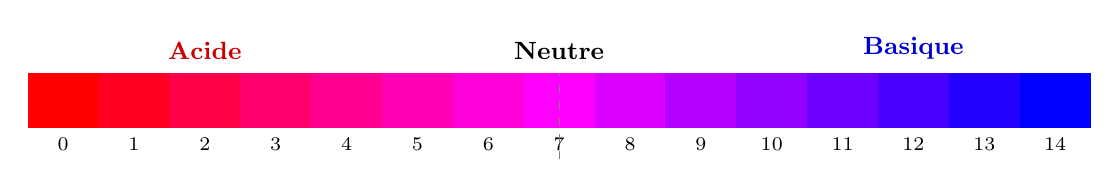
\begin{tikzpicture}[scale=1]
  \foreach \x in {0,...,14} {
    \pgfmathsetmacro{\rval}{max(0,min(1, (14-\x)/7))}
    \pgfmathsetmacro{\bval}{max(0,min(1, \x/7))}
    \definecolor{phcol}{rgb}{\rval,0,\bval}
    \fill[phcol] (\x*0.9,0) rectangle (\x*0.9+0.9,0.7);
    \node[below, font=\scriptsize] at (\x*0.9+0.45, 0) {\x};
  }
  \node[above, font=\small\bfseries, red!80!black] at (2.25, 0.75) {Acide};
  \node[above, font=\small\bfseries, black] at (6.75, 0.75) {Neutre};
  \node[above, font=\small\bfseries, blue!80!black] at (11.25, 0.75) {Basique};
  \draw[dashed, gray] (6.75, -0.4) -- (6.75, 0.7);
\end{tikzpicture}
\end{center}
\vspace{1mm}
\end{docbox}

\vspace{2mm}

\begin{questions}
\begin{enumerate}[label=\textbf{\arabic*.}, leftmargin=*, itemsep=4mm]

\item En vous aidant des documents 3A et 3B :
\begin{enumerate}[label=\alph*), itemsep=2mm]
  \item Classez les 5 produits du tableau par ordre de pH \textbf{croissant}. \pts{1}
  \item Lesquels sont \textbf{acides} ? Lesquels sont \textbf{basiques} ? Lequel est \textbf{neutre} ? \pts{2}
\end{enumerate}

\item Quel produit du tableau est le \textbf{plus dangereux} pour la peau ?\\
Justifiez en vous appuyant sur sa valeur de pH. \pts{2}

\item Un technicien dilue une solution d'acide chlorhydrique de pH $= 1$ en ajoutant de l'eau.
\begin{enumerate}[label=\alph*), itemsep=2mm]
  \item Qu'arrive-t-il au pH lors de la dilution ? \pts{1}
  \item Peut-on obtenir une solution basique en diluant uniquement \`a l'eau ? Expliquez. \pts{2}
\end{enumerate}

\end{enumerate}
\end{questions}

\vspace{8mm}
\begin{center}
  {\color{bleuDNB}\rule{0.6\linewidth}{1pt}}\\[3mm]
  \textit{\textbf{Fin de l'\'epreuve} -- V\'erifiez vos r\'eponses avant de rendre votre copie.}\\[2mm]
  {\color{bleuDNB}\rule{0.6\linewidth}{1pt}}
\end{center}

\end{document}
